\begin{figure}[H]
    \centering
    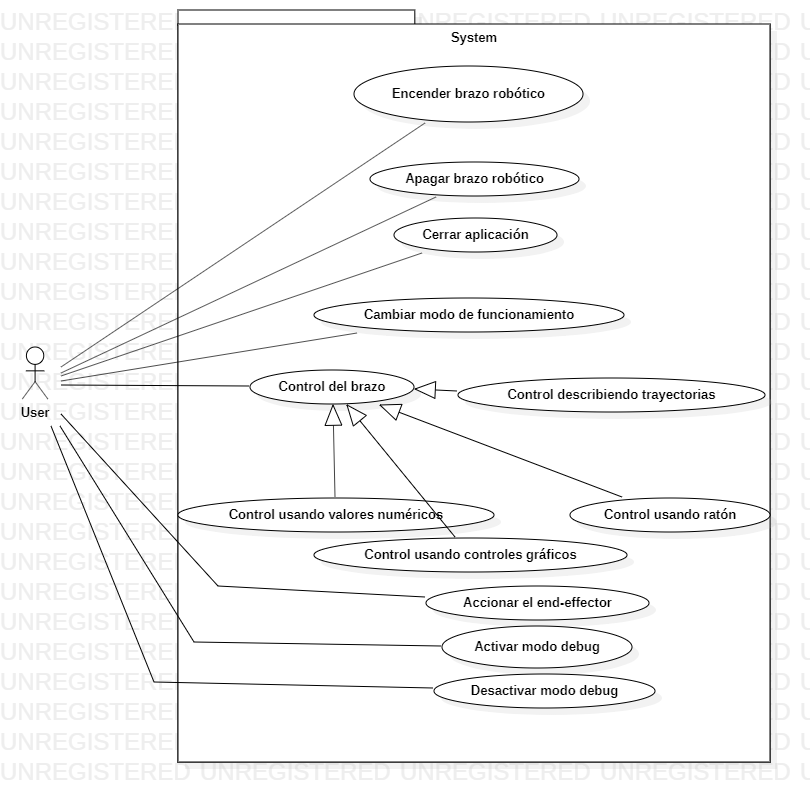
\includegraphics[width=.7\textwidth]{RS/images/UseCaseDiagram1.png}
    \caption{Diagrama de casos de uso}
    \label{fig:diagrama_casos_uso}
\end{figure}


\begin{table}[H]
    \centering
    \begin{tabularx}{\textwidth}{|c|c|X|}
        \cline{1-3}
        \texttt{0001}                              & \multicolumn{2}{c|}{Encender brazo robótico (\ac{S2})}                                                                                                                      \\ \cline{1-3}
        \textbf{Descripción}                       & \multicolumn{2}{m{13cm}|}{El usuario deberá se capaz de encender el sistema del brazo robótico de manera independiente de la aplicación de control.}
        \\ \cline{1-3}
        \multirow{4}{*}{\textbf{Secuencia Normal}} & \textbf{Paso} & \textbf{Acción}
        \\ \cline{2-3}                    &   1  & El usuario interactúa con el sistema para encenderlo.
        \\ \cline{2-3}                    &   2  & El sistema comprueba que los motores están correctamente conectados y que se mueven correctamente hasta el final de carrera.
        \\ \cline{2-3}                    &   3  & Si las comprobaciones son satisfactorias, el sistema continúa con su normal ejecución.
        \\ \cline{1-3}
        \multirow{2}{*}{\textbf{Excepciones}}      & \textbf{Paso}                                                                                                                                        & \textbf{Acción}
        \\ \cline{2-3}                    &   3  & Si las comprobaciones no son satisfactorias el sistema activará un indicador luminoso y se informará del error a \ac{S1}, si está conectado.
        \\ \cline{1-3}
        \textbf{Importancia}                       & \multicolumn{2}{c|}{1}                                                                                                                                                 \\ \cline{1-3}
        \textbf{Comentarios}                       & \multicolumn{2}{c|}{Sin comentarios}                                                                                                                                   \\ \cline{1-3}
    \end{tabularx}
    \caption{Caso de uso \texttt{0001} - Encender brazo robótico (\ac{S2}).}
    \label{tab:CU0001}
    \label{tab:caso_de_uso_encender_brazo_robotico}
\end{table}

\begin{table}[H]
    \centering
    \begin{tabularx}{\textwidth}{|c|c|X|}
        \cline{1-3}
        \texttt{0002}                              & \multicolumn{2}{c|}{Apagar brazo robótico(\ac{S2})}                    \\ \cline{1-3}
        \textbf{Descripción}                       & \multicolumn{2}{m{13cm}|}{El usuario deberá ser capaz de apagar el brazo robótico desconectando la corriente del mismo.}
        \\ \cline{1-3}
        \multirow{4}{*}{\textbf{Secuencia Normal}} & \textbf{Paso}  & \textbf{Acción}
        \\ \cline{2-3}                             &   1            & El usuario interactúa con el sistema para apagarlo.
        \\ \cline{2-3}                             &   2            & El sistema se apaga.
        \\ \cline{1-3}
        \multirow{2}{*}{\textbf{Excepciones}}      & \textbf{Paso}                                                                                                                                        & \textbf{Acción}
        \\ \cline{2-3}                    &     & No existen
        \\ \cline{1-3}
        \textbf{Importancia}                       & \multicolumn{2}{c|}{1}                                                                                                                                                 \\ \cline{1-3}
        \textbf{Comentarios}                       & \multicolumn{2}{c|}{Sin comentarios}                                                                                                                                   \\ \cline{1-3}
    \end{tabularx}
    \caption{Caso de uso \texttt{0002} - Apagar brazo robótico (\ac{S2}).}
    \label{tab:CU0002}
    \label{tab:caso_de_uso_apagar_brazo_robotico}
\end{table}

\begin{table}[H]
    \centering
    \begin{tabularx}{\textwidth}{|c|c|X|}
        \cline{1-3}
        \texttt{0003}        & \multicolumn{2}{c|}{Cerrar aplicación}                                                       
        \\ \cline{1-3}
        \textbf{Descripción} & \multicolumn{2}{m{13cm}|}{El usuario deberá ser capaz de cerrar la aplicación de control de manera independiente al brazo robótico.}
        \\ \cline{1-3}
        \multirow{4}{*}{\textbf{Secuencia Normal}} & \textbf{Paso} & \textbf{Acción}
        \\ \cline{2-3}                    &   1  & El usuario interactúa con la aplicación para cerrarla
        \\ \cline{2-3}                    &   2  & Se comprueba que la  aplicación se puede cerrar de manera segura. Esto implica asegurar que no hay ninguna comunicación en proceso antes de cerrar la aplicación así como que el brazo no se esté moviendo.
        \\ \cline{2-3}                    &   3  & Se realiza el cierre de la aplicación.
        \\ \cline{1-3}
        \multirow{2}{*}{\textbf{Excepciones}} & \textbf{Paso} & \textbf{Acción}
        \\ \cline{2-3}                        &  2  & La aplicación no se puede cerrar de manera segura.
        \\ \cline{2-3}                        & 2.1 & Se impide el cierre
        \\ \cline{1-3}
        \textbf{Importancia}                 & \multicolumn{2}{c|}{1}           
        \\ \cline{1-3}
        \textbf{Comentarios}                 & \multicolumn{2}{c|}{Sin comentarios}
        \\ \cline{1-3}
    \end{tabularx}
    \caption{Caso de uso \texttt{0003} - Cerrar aplicación.}
    \label{tab:CU0003}
    \label{tab:caso_de_uso_cerrar_aplicación}
\end{table}


\begin{table}[H]
    \centering
    \begin{tabularx}{\textwidth}{|c|c|X|}
        \cline{1-3}
        \texttt{0004}                              & \multicolumn{2}{c|}{Cambiar modo de funcionamiento (\ac{S1})}                                                                                                                      \\ \cline{1-3}
        \textbf{Descripción}                       & \multicolumn{2}{m{13cm}|}{El usuario deberá ser capaz de seleccionar el modo de control del brazo robótico, pudiendo escoger entre control mediante ratón o control mediante parámetros. }
        \\ \cline{1-3}
        \multirow{4}{*}{\textbf{Secuencia Normal}} & \textbf{Paso}                                                                                                                                        & \textbf{Acción}
        \\ \cline{2-3}                    &   1  & El usuario interactúa con la aplicación y selecciona el modo de control del robot.
        \\ \cline{2-3}                    &   2  & El sistema cambia entre modo de control mediante ratón o modo de control mediante parámetros.
        \\ \cline{1-3}
        \multirow{2}{*}{\textbf{Excepciones}}      & \textbf{Paso}                                                                                                                                        & \textbf{Acción}
        \\ \cline{2-3}                    &     &  No existen
        \\ \cline{1-3}
        \textbf{Importancia}                       & \multicolumn{2}{c|}{1}                                                                                                                                                 \\ \cline{1-3}
        \textbf{Comentarios}                       & \multicolumn{2}{c|}{Sin comentarios}                                                                                                                                   \\ \cline{1-3}
    \end{tabularx}
    \caption{Caso de uso \texttt{0004} - Cambiar modo de funcionamiento.}
    \label{tab:CU0004}
    \label{tab:caso_de_uso_cambiar_modo_de_funcionamiento}
\end{table}


\begin{table}[H]
    \centering
    \begin{tabularx}{\textwidth}{|c|c|X|}
        \cline{1-3}
        \texttt{0005}                              & \multicolumn{2}{c|}{Control usando valores numéricos (\ac{S1})}                                                                                                                      \\ \cline{1-3}
        \textbf{Descripción}                       & \multicolumn{2}{m{13cm}|}{El usuario deberá ser capaz de cambiar el valor numérico de cada uno de los parámetros de control del brazo robótico}
        \\ \cline{1-3}
        \multirow{4}{*}{\textbf{Secuencia Normal}} & \textbf{Paso}                                                                                                                                        & \textbf{Acción}
        \\ \cline{2-3}                    &   1  & El usuario interactúa con la aplicación y cambia el valor de los parámetros de control usando el teclado.
        \\ \cline{2-3}                    &   2  & Se comprueba si el valor es correcto y se confirma el cambio del valor numérico.
        \\ \cline{1-3}
        \multirow{2}{*}{\textbf{Excepciones}} & \textbf{Paso}  & \textbf{Acción}
        \\ \cline{2-3}                        &   2  & El valor introducido por el usuario no es correcto y por lo tanto no puede llevarse a la práctica.
        \\ \cline{2-3} 
                                              &  2.1 & Se elimina el valor y se notifica al usuario sobre el error y se le pide que introduzca de nuevo el valor.
        \\ \cline{1-3}
        \textbf{Importancia}                       & \multicolumn{2}{c|}{1}                                                                                                                                                 \\ \cline{1-3}
        \textbf{Comentarios}                       & \multicolumn{2}{c|}{Sin comentarios}                                                                                                                                   \\ \cline{1-3}
    \end{tabularx}
    \caption{Caso de uso \texttt{0005} - Control usando valores numéricos (\ac{S1}).}
    \label{tab:CU0005}
    \label{tab:caso_de_uso_control_usando_valores_numericos}
\end{table}

\begin{table}[H]
    \centering
    \begin{tabularx}{\textwidth}{|c|c|X|}
        \cline{1-3}
        \texttt{0006}        & \multicolumn{2}{c|}{Control describiendo trayectorias}                                      
        \\ \cline{1-3}
        \textbf{Descripción} & \multicolumn{2}{m{13cm}|}{Se permitirá al usuario escoger una trayectoria predefinida que el brazo robótico deberá realizar.}
        \\ \cline{1-3}
        \multirow{4}{*}{\textbf{Secuencia Normal}} & \textbf{Paso} & \textbf{Acción}
        \\ \cline{2-3}                    &   1  & El usuario selecciona una trayectoria a realizar.
        \\ \cline{2-3}                    &   2  & Se realiza dicha trayectoria
        \\ \cline{1-3}
        \multirow{2}{*}{\textbf{Excepciones}} & \textbf{Paso} & \textbf{Acción}
        \\ \cline{2-3}                    &      &  No existen
        \\ \cline{1-3}
        \textbf{Importancia}                 & \multicolumn{2}{c|}{1}           
        \\ \cline{1-3}
        \textbf{Comentarios}                 & \multicolumn{2}{m{13cm}|}{\textbf{Esta característica no se implementa ya que se posterga para una futura versión.}}
        \\ \cline{1-3}
    \end{tabularx}
    \caption{Caso de uso \texttt{0006} - Control describiendo trayectorias.}
    \label{tab:CU0006}
    \label{tab:caso_de_uso_control_describiendo_trayectorias}
\end{table}

\begin{table}[H]
    \centering
    \begin{tabularx}{\textwidth}{|c|c|X|}
        \cline{1-3}
        \texttt{0007}        & \multicolumn{2}{c|}{Control usando controles gráficos}                                      
        \\ \cline{1-3}
        \textbf{Descripción} & \multicolumn{2}{m{13cm}|}{La interfaz gráfica de la aplicación debe ofrecer control sobre los parámetros del brazo robótico mediante \textit{sliders}.}
        \\ \cline{1-3}
        \multirow{4}{*}{\textbf{Secuencia Normal}} & \textbf{Paso} & \textbf{Acción}
        \\ \cline{2-3}                    &   1  & El usuario interactúa con la aplicación y mueve los \textit{sliders} para variar los parámetros del brazo robótico.
        \\ \cline{2-3}                    &   2  & Se verifica si se puede realizar dicho movimiento y se ejecuta el cambio en los parámetros.
        \\ \cline{1-3}
        \multirow{2}{*}{\textbf{Excepciones}} & \textbf{Paso} & \textbf{Acción}
        \\ \cline{2-3}                    &   2   &  La posición no es alcanzable o no se puede llevar a la práctica.
        \\ \cline{2-3}                    &  2.1  &  Se notifica el error.
        \\ \cline{1-3}
        \textbf{Importancia}                 & \multicolumn{2}{c|}{1}           
        \\ \cline{1-3}
        \textbf{Comentarios}                 & \multicolumn{2}{c|}{Sin comentarios}
        \\ \cline{1-3}
    \end{tabularx}
    \caption{Caso de uso \texttt{0007} - Control usando controles gráficos.}
    \label{tab:CU0007}
    \label{tab:caso_de_uso_control_usando_controles_graficos}
\end{table}

\begin{table}[H]
    \centering
    \begin{tabularx}{\textwidth}{|c|c|X|}
        \cline{1-3}
        \texttt{0008}        & \multicolumn{2}{c|}{Control usando ratón}                                      
        \\ \cline{1-3}
        \textbf{Descripción} & \multicolumn{2}{m{13cm}|}{Se permitirá al usuario controlar el brazo robótico de manera directa con el movimiento del ratón}
        \\ \cline{1-3}
        \multirow{4}{*}{\textbf{Secuencia Normal}} & \textbf{Paso} & \textbf{Acción}
        \\ \cline{2-3}                    &   1  & El usuario mueve el ratón realizando movimientos libres.
        \\ \cline{2-3}                    &   2  & Se comprueba que el movimiento no se sale de los margenes permitidos
        \\ \cline{2-3}                    &   3  & Se realiza el movimiento
        \\ \cline{1-3}
        \multirow{2}{*}{\textbf{Excepciones}} & \textbf{Paso} & \textbf{Acción}
        \\ \cline{2-3}                    &   2   &  Si los movimientos se salen de los margenes permitidos no se realizan.
        \\ \cline{1-3}
        \textbf{Importancia}                 & \multicolumn{2}{c|}{1}           
        \\ \cline{1-3}
        \textbf{Comentarios}                 & \multicolumn{2}{m{13cm}|}{\textbf{Esta característica no se implementa ya que se posterga para una futura versión.}}
        \\ \cline{1-3}
    \end{tabularx}
    \caption{Caso de uso \texttt{0008} - Control usando ratón.}
    \label{tab:CU0008}
    \label{tab:caso_de_uso_control_usando_ratón}
\end{table}

\begin{table}[H]
    \centering
    \begin{tabularx}{\textwidth}{|c|c|X|}
        \cline{1-3}
        \texttt{0009}        & \multicolumn{2}{c|}{Accionar el \textit{end--effector}}                                      
        \\ \cline{1-3}
        \textbf{Descripción} & \multicolumn{2}{m{13cm}|}{Se permite al usuario abrir y cerrar la pinza}
        \\ \cline{1-3}
        \multirow{4}{*}{\textbf{Secuencia Normal}} & \textbf{Paso} & \textbf{Acción}
        \\ \cline{2-3}                    &   1  & El usuario interactúa con la aplicación para abrir y cerrar el \textit{end--effector}
        \\ \cline{2-3}                    &   2  & Se cambia el estado del \textit{end--effector} según sea necesario. 
        \\ \cline{1-3}
        \multirow{2}{*}{\textbf{Excepciones}} & \textbf{Paso} & \textbf{Acción}
        \\ \cline{2-3}                    &      &  No existe
        \\ \cline{1-3}
        \textbf{Importancia}                 & \multicolumn{2}{c|}{1}           
        \\ \cline{1-3}
        \textbf{Comentarios}                 & \multicolumn{2}{m{13cm}|}{\textbf{Esta característica no se implementa ya que se posterga para una futura versión.}}
        \\ \cline{1-3}
    \end{tabularx}
    \caption{Caso de uso \texttt{0009} - Accionar el \textit{end--effector}.}
    \label{tab:CU0009}
    \label{tab:caso_de_uso_accionar_end_effector}
\end{table}

\begin{table}[H]
    \centering
    \begin{tabularx}{\textwidth}{|c|c|X|}
        \cline{1-3}
        \texttt{0010}        & \multicolumn{2}{c|}{Activar modo \textit{debug}}                                      
        \\ \cline{1-3}
        \textbf{Descripción} & \multicolumn{2}{m{13cm}|}{Se permite al usuario activar un modo tal que se pueda mandar al \ac{S2} el código de control del brazo robótico}
        \\ \cline{1-3}
        \multirow{4}{*}{\textbf{Secuencia Normal}} & \textbf{Paso} & \textbf{Acción}
        \\ \cline{2-3}                    &   1  & El usuario interactúa con S2 para ponerlo en modo debug.
        \\ \cline{2-3}                    &   2  & El sistema comprueba que el cambio de modo se puede hacer de manera segura. Es decir, no hay una comunicación específica del modo de funcionamiento actual en proceso antes de realizar el cambio.
        \\ \cline{2-3}                    &   3  & El sistema cambia de modo.
        \\ \cline{1-3}
        \multirow{2}{*}{\textbf{Excepciones}} & \textbf{Paso} & \textbf{Acción}
        \\ \cline{2-3}                    &   2  & El sistema detecta que el cambio de modo no se puede hacer de manera segura e impide que este se realice. Se informará del error a \ac{S1}, si está conectado.
        \\ \cline{1-3}
        \textbf{Importancia}                 & \multicolumn{2}{c|}{1}           
        \\ \cline{1-3}
        \textbf{Comentarios}                 & \multicolumn{2}{m{13cm}|}{\textbf{Esta característica no se implementa ya que se posterga para una futura versión.}}
        \\ \cline{1-3}
    \end{tabularx}
    \caption{Caso de uso \texttt{0010} - Activar el modo \textit{debug}.}
    \label{tab:CU0010}
    \label{tab:caso_de_uso_activar_modo_debug}
\end{table}

\begin{table}[H]
    \centering
    \begin{tabularx}{\textwidth}{|c|c|X|}
        \cline{1-3}
        \texttt{0011}        & \multicolumn{2}{c|}{Desactivar modo \textit{debug}}                                      
        \\ \cline{1-3}
        \textbf{Descripción} & \multicolumn{2}{m{13cm}|}{Se permite al usuario desactivar el modo debug tal que sea posible emplear el sistema de manera normal}
        \\ \cline{1-3}
        \multirow{4}{*}{\textbf{Secuencia Normal}} & \textbf{Paso} & \textbf{Acción}
        \\ \cline{2-3}                    &   1  & El usuario interactúa con \ac{S2} para desactivar el modo debug.
        \\ \cline{2-3}                    &   2  & El sistema comprueba que el cambio de modo se puede hacer de manera segura.
        \\ \cline{2-3}                    &   3  & El sistema cambia de modo.
        \\ \cline{1-3}
        \multirow{2}{*}{\textbf{Excepciones}} & \textbf{Paso} & \textbf{Acción}
        \\ \cline{2-3}                    &   2  & El sistema detecta que el cambio de modo no se puede hacer de manera segura e impide que este se realice. Se informara del error a \ac{S1}, si esta conectado.
        \\ \cline{1-3}
        \textbf{Importancia}                 & \multicolumn{2}{c|}{1}           
        \\ \cline{1-3}
        \textbf{Comentarios}                 & \multicolumn{2}{m{13cm}|}{\textbf{Esta característica no se implementa ya que se posterga para una futura versión.}}
        \\ \cline{1-3}
    \end{tabularx}
    \caption{Caso de uso \texttt{0011} - Desactivar el modo \textit{debug}.}
    \label{tab:CU0011}
    \label{tab:caso_de_uso_desactivar_modo_debug}
\end{table}